\chapter{Metodología}

\section{Modelos matemáticos}

De acuerdo con \cite{Dombre2007}, el diseño y control de robots requiere diversos modelos matemáticos, tales como:

\begin{itemize}
\itemsep0em 

\item Cinemática directa e inversa, es decir, encontrar la posición del efector final en términos de las coordenadas de las articulaciones y viceversa.
\item Cinemática de la velocidad, encontrar la velocidad del efector final en términos de la velocidad de las articulaciones y viceversa.
\item Modelo dinámico, el cual establece la relación entre los torques o fuerzas que ejercen los actuadores y las posiciones, velocidades y aceleraciones de las articulaciones.
\end{itemize}

\begin{figure}
    \centering
    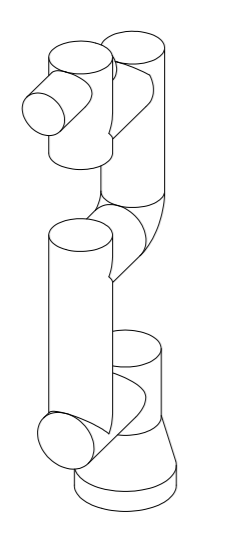
\includegraphics[scale=0.7]{./img/chapter4/robotarmprototype.png}
    \caption{Boceto del brazo robótico propuesto}
    \label{fig:roboticarmprototype}
\end{figure}

En este capítulo se desarrollarán los modelos matemáticos necesarios para simular y diseñar el brazo robótico, así como predecir el comportamiento del mismo.

Para realizar estos modelos, es importante contar con los parámetros físicos y geométricos del robot, los cuales aún no están completamente definidos, por lo que, para una primera aproximación, se utilizarán valores experimentales. Éstos se mencionan en la tabla \ref{table:parametrosbrazorobotico}.

Otros parámetros necesarios para el desarrollo del modelo matemático del brazo robótico son el alcance total del brazo, el cual deberá ser de mínimo 500 mm, la velocidad, la cuál deberá estar en un rango entre 5 RPM y 30 RPM, y por último, la carga útil, la cuál deberá ser de 2 kg.

\begin{table}
\centering
\caption{Parámetros del brazo robótico}
 \label{table:parametrosbrazorobotico}
\begin{tabular}{l|l|l|l|l|l|l|}
\textbf{Eslabones}                       &  1   &  2   &  3   &  4   &  5   &  6    \\ 
\hline
Longitud           & 0.152       & 0.104       & 0.244       & 0.104       & 0.213       & 0.104        \\
Masa               & 0           & 2           & 1           & 0.8         & 0.8         & 0.2          \\
Centro de gravedad & {[}0, 0, 0] & {[}0, 0, 0] & {[}0, 0, 0] & {[}0, 0, 0] & {[}0, 0, 0] & {[}0, 0, 0]  \\
Matriz de inercia      & {[}0, 0, 0] & {[}0, 0, 0] & {[}0, 0, 0] & {[}0, 0, 0] & {[}0, 0, 0] & {[}0, 0, 0]  \\
Fricción en eslabón    & 0.00148     & 0.00817     & 0.00138     & 7.12e-05    & 8.26e-05    & 3.67e-05     \\
Fricción de Coulomb    & 0.395       & 0.126       & 0.132       & 0.0113      & 0.00926     & 0.00396      \\
Inercia del motor      & 0.002       & 0.002       & 0.002       & 3.3e-05     & 3.3e-05     & 3.3e-05     
\end{tabular}
\end{table}

En la figura \ref{fig:roboticarmprototype} podemos ver un boceto del brazo robótico que se planea implementar.

Con estos datos definidos, es posible empezar la realización de los modelos matemáticos.

\subsection{Cinemática directa e inversa.}

En esta sección se desarrollará el primer modelo matemático del brazo robótico, la cinemática directa e inversa, la cual se trata de encontrar la posición final del brazo dependiendo de las coordenadas $\theta$ de sus articulaciones o, para el caso de la cinemática inversa, calcular las coordenadas $\theta$ necesarias para llegar a una posición $(x,y,z)$ dada.

\subsubsection{Cinemática directa} 
Como ya se mencionó anteriormente, la cinemática directa de un brazo robótico se refiere al cálculo de la posición y orientación del marco de referencia del efector final a partir de las coordenadas $\theta$ de sus articulaciones. \cite{University2017}

Un ejemplo de esto lo podemos encontrar en la figura \ref{fig:forwardkinematic2}, donde se analiza la cinemática directa de un brazo robótico de tres grados de libertad. En este ejemplo podemos apreciar que la longitud de los eslabones se representan como $L_1, L_2, L_3$ respectivamente y se ha escogido un marco de referencia fijo denominado \{0\}, mientras que el marco de referencia del efector final es \{4\}. \cite{University2017}

Entonces, para conocer la posición final es necesaria la siguente ecuación:
\begin{equation}\\
\label{eq:cinematicadirecta1}
x = L_1 \cos(\theta_1)+L_2 \cos(\theta_1 + \theta_2)+ L_3 \cos(\theta_1 + \theta_2 + \theta_3)
\end{equation}
\begin{equation}
\label{eq:cinematicadirecta2}
y = L_1 \sin(\theta_1)+L_2 \sin(\theta_1 + \theta_2)+ L_3 \sin(\theta_1 + \theta_2 + \theta_3)
\end{equation}
\begin{equation}
\label{eq:cinematicadirecta3}
\phi = \theta_1 + \theta_2 + \theta_3
\end{equation}

Las ecuaciones \ref{eq:cinematicadirecta1}, \ref{eq:cinematicadirecta2} y \ref{eq:cinematicadirecta3} se les conoce como \textbf{ecuación de cinemática directa} y aunque es válida, se vuelve rápidamente compleja para un brazo robótico de seis grados de libertad, por esta razón, el enfoque sistemático de resolución es utilizar matrices de transformación homogenea y la convención de Denavit-Hartenberg.

\begin{figure}
    \centering
    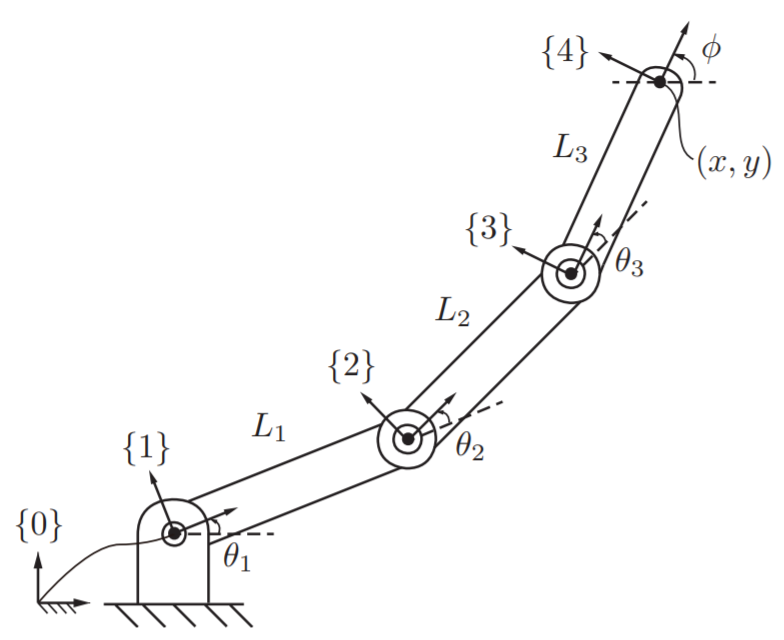
\includegraphics[scale=0.6]{./img/chapter3/forwardkinematic.png}
    \caption{Cinemática directa de un brazo robótico de 3 grados de libertad \cite{University2017}}
    \label{fig:forwardkinematic2}
\end{figure}

\paragraph{Matriz de transformación homogénea.}

Una matriz de transformación homogenea no es nada más que la representación matricial de un movimiento rígido \cite{Spong2005}, así, la posición y orientación del efector final puede ser fácilmente calculada utilizando multiplicación de matrices.


Según \cite{University2017}, existen tres usos principales para una matriz de transformación homogénea:

\begin{enumerate}
\itemsep0em
  \item Para representar la configuración (posición y orientación) de un cuerpo rígido.
  \item Para cambiar el marco de referencia en el cuál está representado un vector u otro marco de referencia.
  \item Para desplazar un vector o un marco de referencia.
\end{enumerate}

Para el caso que nos ocupa, necesitamos la matriz de transformación homogénea desde la base fija del robot hasta su efector final, descrita con la ecuación siguiente:
\begin{equation}
\label{eq:homogeneustransformationmatrix}
\begin{split}
{}_{0}^{7}T = \mathscr{T}_z(a_1)\oplus\mathscr{R}_z(\theta_1)\oplus\mathscr{T}_x(b_1)\oplus\mathscr{R}_x(\theta_2)\oplus\mathscr{T}_z(c_1)\oplus\mathscr{R}_x(\theta_3) \\ \oplus\mathscr{T}_z(d_1)\oplus\mathscr{T}_x(d_2)\oplus\mathscr{R}_x(\theta_4)\oplus\mathscr{T}_x(e_1)\oplus\mathscr{R}_z(\theta_5)\oplus\mathscr{T}_z(f_1)\oplus\mathscr{R}_x(\theta_6)
\end{split}
\end{equation}

Dónde $a_1, b_1, c_1, d_1, d_2, e_1$ y $f_1$ son las longitudes de los eslabones del brazo robótico. 

\begin{figure}
    \centering
    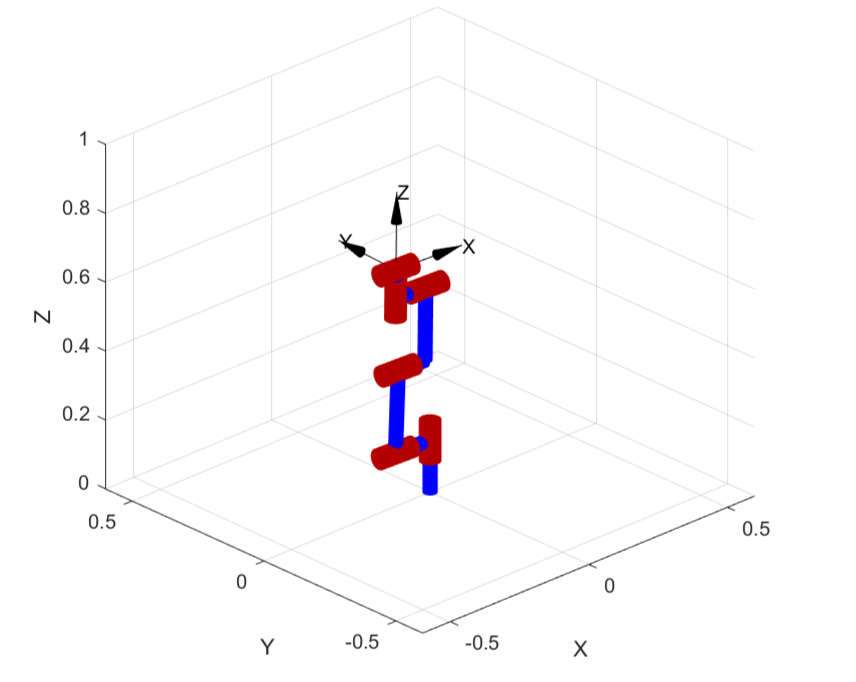
\includegraphics[scale=0.6]{./img/chapter4/KinematicDiagramML.png}
    \caption{Cadena cinemática}
    \label{fig:kinematicchain}
\end{figure}


En la imagen \ref{fig:kinematicchain} podemos observar la cadena cinemática de nuestro brazo robótico, fue creada con un algoritmo en MATLAB con ayuda de la herramienta Robotic Toolbox \cite{Corke2017}, dicho código puede consultarse en el Anexo 1.


\paragraph{Convención de Denavit-Hartenberg.} En muchas aplicaciones, es necesario representar los parámetros cinemáticos de forma simplificada con ayuda de la notación Denavit-Hartenberg, con esta convención se simplifa considerablemente el análisis.

Con esta notación podemos hacer uso de algoritmos de solución para encontrar los valores dinámicos, planeación de trayectorias y simulaciones, entre otros valores.

En \cite{Corke2007}, se propone un acercamiento sencillo y sistemático para convertir una matriz de transformación homogenea como la de la ecuación \ref{eq:homogeneustransformationmatrix} en los parámetros de Denavit-Hartenberg. 

Al realizar dicho proceso se llegó a los resultados que se muestran en la tabla \ref{table:denavithartenberg}.

\begin{table}
\centering
\caption{Parámetros Denavit Hartenberg}
 \label{table:denavithartenberg}
\begin{tabular}{l|l|l|l|l|}
               & $\theta$ [rad] & d [m]    & a [m]   & $\alpha$ [rad]                        \\ 
\hline
Articulación 1 & $\theta_1$              & 0.152    & 0       & $\frac{\pi}{2}$   \\
Articulación 2 & $\theta_2$              & 0        & -0.244       & 0 \\
Articulación 3 & $\theta_3$                  & 0 & -0.213       & 0                                                  \\
Articulación 4 & $\theta_4$              & -0.012        & 0 & $-\frac{\pi}{2}$   \\
Articulación 5 & $\theta_5$                        & 0.085        & 0 & $\frac{\pi}{2}$  \\
Articulación 6 & $\theta_6$                           & 0        & 0  & $-\frac{\pi}{2}$                                                 
\end{tabular}
\end{table}

Con esto, tenemos una vista simplificada de nuestro brazo robótico, que describe su cinemática directa usando únicamente cuatro parámetros por articulación. El algoritmo desarrollado puede consultarse en el Anexo 2.	

\subsubsection{Cinemática inversa}

Una vez terminada la cinemática directa, toca al turno de abordar la cinemática inversa. Hasta este punto podemos calcular la posición del efector final utilizando las variables de las articulaciones, ahora, procederemos a encontrar las variables de las articulaciones dada una posición y orientación del efector final.

Para nuestro caso, un brazo robótico de seis grados de libertad, la solución tiene doce ecuaciones con seis incognitas, sin embargo, nueve ecuaciones se derivan de la matriz de rotación dentro de la matriz de transformación homogenea ${}_{0}^{6}T$, esto deja unicamente tres ecuaciones independientes, agregando las tres ecuaciones del vector de posición dentro de la matriz de transformación homogenea ${}_{0}^{6}T$ nos da como resultado seis ecuaciones con seis incógnitas.	

Estas ecuaciones son no-lineales y transendentales, lo cual hace más dificil encontrar una solución y como cualquier conjunto de ecuaciones no-lineales, puede existir una sola solución o múltiples soluciones. \cite{Craig2013}

Para resolver el problema de encontrar la cinemática inversa existen dos métodos posibles: \textit{la solución de forma cerrada} y la solución numérica. 

El concenso de la mayoría de los autores, tales como \cite{Spong2005} y \cite{Craig2013} es que se prefiere encontrar la solución de forma cerrada por dos razones principales, la velocidad de solución y la forma en la que se encuentra una solución, es decir, como la cinemática inversa puede tener muchas soluciones se pueden desarrollar reglas para favorecer un tipo de solución con respecto de otra.

Queda claro que resolver la cinemática inversa no es tarea sencilla, por esta razón y de manera parecida a como se manejó en la sección anterior, se utilizará la librería Robotic Toolbox, la cual incluye un método establecido para calcular la cinemática inversa dada una matriz de transformación homogénea. El algoritmo desarrollado puede consultarse en el Anexo 3.

Así mismo, es importante notar que esta solución se utilizará únicamente en la etapa de desarrollo del brazo robótico y se tendrá que implementar un algoritmo de solución de cinemática inversa en el control final del robot.

\subsection{Cinemática de la velocidad}

Soon.

\subsection{Modelo dinámico}

Hasta ahora, se ha descrito el movimiento del robot sin consideración de las fuerzas y los torques necesarios para producir dicho movimiento, ahora toca el turno de analizarlas.

Como se comentó al principio del capítulo, es necesario establecer una relación entre las posiciones, velocidades y aceleraciones deseadas y el torque o fuerzas que se debe ejercer en los actuadores, esto nos permitirá controlar el brazo robótico así como conocer los parámetros necesarios que los actuadores deben cumplir para satisfacer los requerimientos de velocidad y carga útil.

Para lograrlo, existen dos fomulaciones que se pueden seguir, la formulación Euler-Lagrange o la formulación Newton-Euler. Ambos métodos llegarían a la misma respuesta, sin embargo el camino será diferente.

En la formulación Euler-Lagrange se trata al robot como un todo y se realiza el análisis utilizando la formulación Lagraniana (la diferencia entre energía cinética y energía potencial), por su parte, la formulación Newton-Euler divide el manipulador en cada uno de sus eslabones y describe las escuaciones que definen su movimiento lineal y angular. \cite{Spong2005}

En esta parte de la investigación y como parte de los modelos matemáticos necesarios para seguir diseñando el robot, se utilizará la \textit{formulación Newton-Euler} para obtener los torques y fuerzas necesarias. 

\subsubsection{Formulación Newton-Euler}

Para encontrar los torques a los que deben estar sometidos las articulaciones del brazo robótico se utilizará la herramienta que se ha utilizado a lo largo de este capítulo, con ella, se desarrolla un algoritmo en MATLAB donde se incluiyen los parámetros necesarios para el modelo dinámico tales como masa, centro de gravedad, momento de inercia, fricción viscosa, fricción de Coulomb, inercia del motor y relación de engranes. 

La lista de parámetros para cada articulación y eslabón fue descrita anteriormente en el cuadro \ref{table:parametrosbrazorobotico}.

Cabe destacar que algunos de los parámetros dinámicos son una aproximación optimista, esto debido a no tener aún un diseño final ni todos los componentes seleccionados, sin embargo, es funcional para una primera iteración del torque necesario para continuar con la selección de componentes.

Con los datos del cuadro \ref{table:parametrosbrazorobotico} se selecciona los torques máximos en el escenario más demandante, esto es en una trayectoria en la cuál cada una de las articulaciones se somete a una mayor fuerza.

Con todos los datos correctamente particularizados, obtenemos una lista con todos los valores máximos, se puede apreciar en el cuadro \ref{table:maxtorque}. 

\begin{table}
\centering
\caption{Parámetros del brazo robótico}
\label{table:maxtorque}
\begin{tabular}{l|l|l|l|l|l|l|}
\textbf{Articulaciones}              &  1 & 2 & 3 &  4 &  5 &  6  \\ 
\hline
Torque máximo & 0.2            & 25.35          & 11.94~         & 2.33           & 0.2            & 0.2            
\end{tabular}
\end{table}

El algoritmo realizado está disponible para consulta en el Anexo 4. Así como el repositorio de esta tésis.
       
\section{Componentes electrónicos}

Aquí necesito seis motores, tres ODrive, seis encoders
Una fuente de poder 

\section{Componentes mecánicos}

Una vez determinado los componentes electrónicos necesarios para el correcto funcionamiento del brazo robótico es necesario determinar los componentes mecánicos.

\section{Actuador}

Una de las partes mecánicas más importantes es el actuador, es decir, el mecanismo que proporcionará la fuerza necesaria para mover las articulaciones del robot.

Para la correcta selección o desarrollo del actuador necesitamos dos parámetros que vimos en los capítulos anteriores, el primero es el torque necesario para realizar los desplazamientos del robot a la velocidades y aceleraciones requeridas y el segundo es la velocidad nominal del motor a utilizar.

Por norma general, los motores eléctricos y, para nuestro caso, los motores eléctricos sin escobillas, funcionan a velocidades altas y un torque relativamente pequeño, para esto es necesario utilizar reductores de velocidad, los cuales cumplen dos objetivos primordiales: reducir la velocidad en eje de salida y aumentar el torque en el mismo.

El siguiente paso es escoger un reductor de velocidad que cumpla con los requerimientos específicos de nuestro brazo robótico, los cuales son:

\begin{itemize}
\item Alta relación de transmisión, mayor a 10:1.
\item Precisión, necesaria para realizar los movimientos deseados sin demasiado juego. 
\item Efectividad de transmisión, necesaria para no perder demasiada energía
\end{itemize}

Estos son algunos de los más importantes, existen otros factores a considerar como el tamaño final del reductor y la facilidad de manufactura.

Para el desarrollo de este brazo robótico se han considerado tres diferentes tipos de reductores de velocidad, cada uno con ventajas y desventajas que se mencionarán a continuación.

\subsection{Engranes planetarios}

El primero en esta lista es un reductor con engranes planetarios, 

Existen proyectos como el de [insertar cita despúes] OpenTorque Actuator de Gabrael Levine que utiliza engranes planetarios en el diseño de su actuador, logra una relación de transmisión de 8:1

En la imagen \ref{fig:opentorque} podemos apreciar su diseño con engranes planetarios del tipo  helicoidal así como una carcasa para el sistema de motor y actuador. 

\begin{figure}[h]
    \centering
    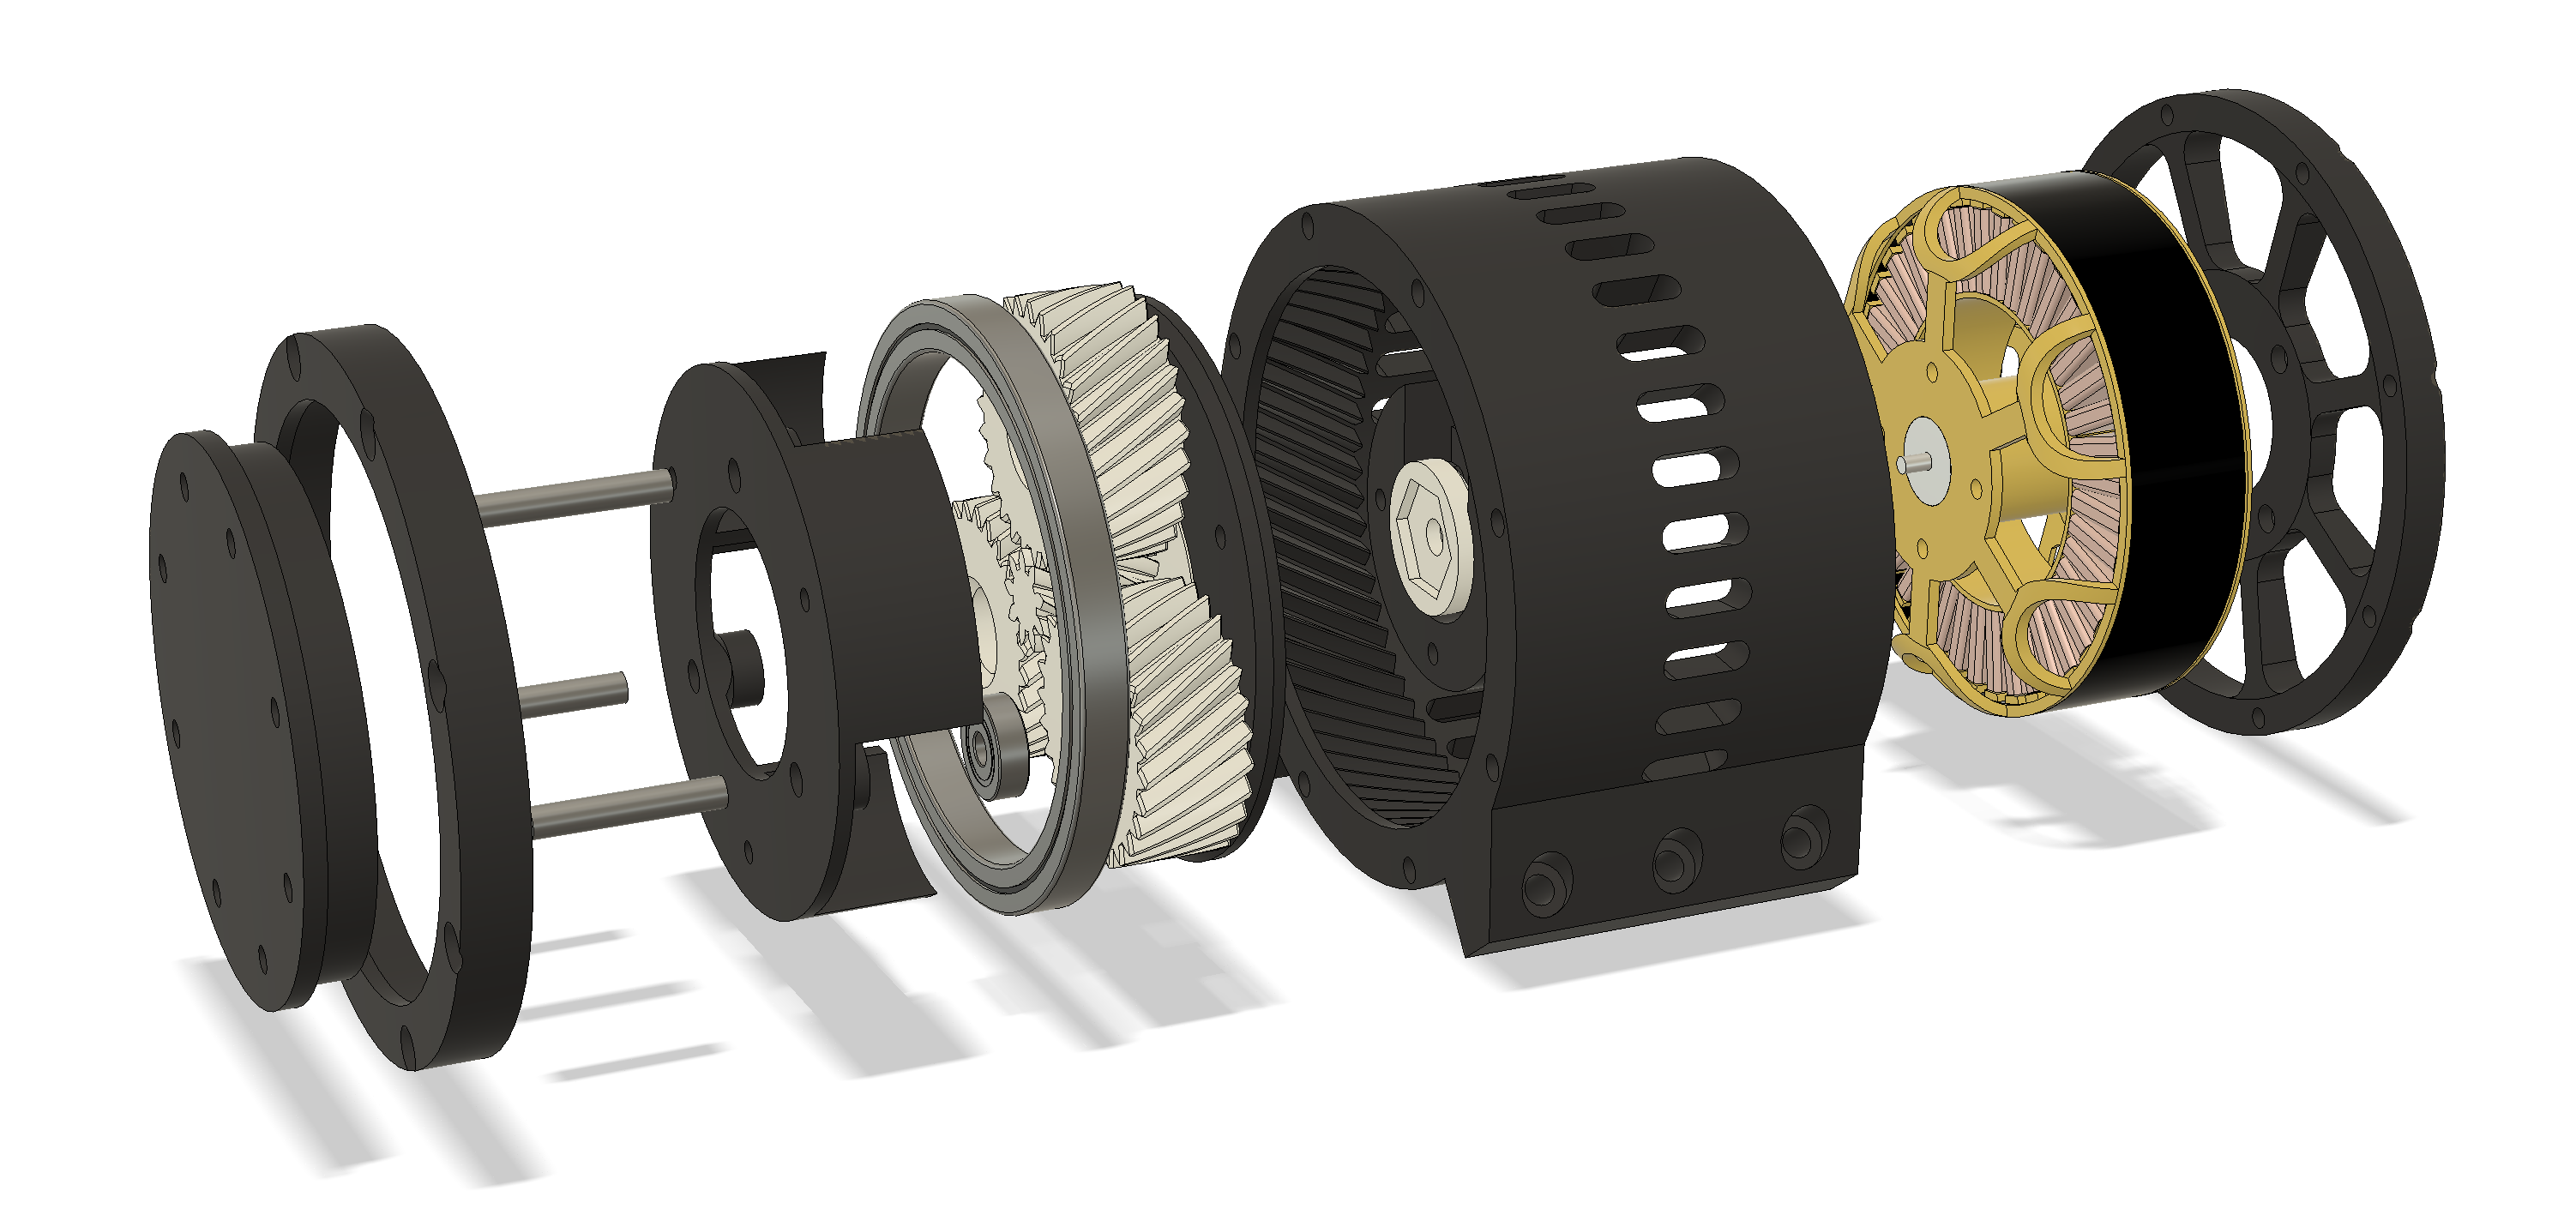
\includegraphics[width=15cm, height=6cm, keepaspectratio]{./img/chapter6/opentorque.png}
    \caption{OpenTorque Actuator por Gabrael Levine}
    \label{fig:opentorque}
\end{figure}

En esta propuesta la ventaja es la relativa facilidad de fabricación con tecnología de manufactura aditiva así como un tamaño y peso considerablemente pequeño.

Las desventajas son su relativamente pequeño relación de transmisión y su poca eficiencia de transmisión.

\subsection{Engrane cicloidal}
\subsection{Harmonic Drive}

  